\titre{}
\theme{Calcul différentiel}
\auteur{Nathan Scheinmann}
\niveau{3M}
\source{}
\type{serie}
\piments{}
\pts{}
\annee{2526}

\contenu{
	\tcblower
	Une fonction $f$ admet le graphe suivant pour $x\in \interval{-1}{11}$.
% Écrivez l'énoncé de l'exercice ici
\begin{center}
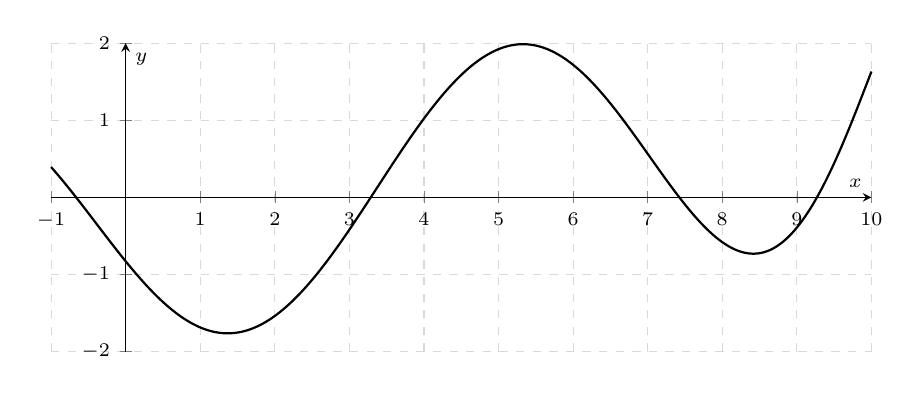
\begin{tikzpicture}[scale=1]
  \begin{axis}[
    width=12cm,      % <–– controls the *axis* width
    height=5.5cm, 
    axis lines=middle,
    % place x‐label at right end of axis:
    xlabel={\scriptsize$x$},
    xlabel style={at={(axis description cs:1,0)},anchor=west},
    % place y‐label at top end of axis:
    ylabel={\scriptsize$y$},
    ylabel style={at={(axis description cs:0,1)},anchor=south},
    axis x line=middle, axis y line=middle,
    every axis x line/.append style={->,>={Stealth[length=3pt]}},
    every axis y line/.append style={->,>={Stealth[length=3pt]}},
    xmin=-1, xmax=10,
    ymin=-2, ymax=2,
    xticklabel style={font=\scriptsize},
    % only y‐ticks (if you ever want it):
    yticklabel style={font=\scriptsize},
    xtick={-1,...,10}, ytick={-2,...,2},
    grid=both,
    grid style={dashed,gray!30},
    clip=false,
  ]
    % 1) f(x) = 1/x – 4 on [–8,–4]

\addplot[smooth, thick, domain=-1:10, samples=400] 
{ -0.000043*x^7 
  + 0.001063*x^6 
  - 0.006601*x^5 
  - 0.013552*x^4 
  + 0.157565*x^3 
  + 0.194188*x^2 
  - 1.190585*x 
  - 0.827667 };

  \end{axis}
\end{tikzpicture}
\end{center}
\begin{tasks}
	\task Pour chaque $a\in \{-2;0;4;6;8\}$, tracer la tangente au graphe de $f$ en son point d'abscisse $a$ puis estimer $f(a)$ et $f'(a)$. 
	\task Estimer graphiquement les solutions des équations suivantes.
	\begin{multicols}{3}
		\begin{enumerate}
			\item $f(x)=0$
			\item $f'(x)=0$
			\item $f(x)=1$
			\item $f'(x)=1$
		\end{enumerate}
	\end{multicols}
\end{tasks}

}
\correction{
% Écrivez la correction ici

}
